\documentclass[12pt,a4paper]{article}
\usepackage{amsmath,,amsbsy,amssymb,latexsym,url,bm,amsthm}
\usepackage{epsfig,graphicx,subfigure}
\usepackage{enumitem,balance}
\usepackage{wrapfig}
\usepackage{mathrsfs,euscript}
\usepackage[usenames]{xcolor}
\usepackage{hyperref}
\usepackage[vlined,ruled,linesnumbered]{algorithm2e}
\hypersetup{colorlinks=true,linkcolor=black}

\newtheorem{theorem}{Theorem}
\newtheorem{lemma}[theorem]{Lemma}
\newtheorem{proposition}[theorem]{Proposition}
\newtheorem{corollary}[theorem]{Corollary}
\newtheorem{exercise}{Exercise}
\newtheorem*{solution}{Solution}
\newtheorem{definition}{Definition}
\theoremstyle{definition}

\renewcommand{\thefootnote}{\fnsymbol{footnote}}

\newcommand{\postscript}[2]
 {\setlength{\epsfxsize}{#2\hsize}
  \centerline{\epsfbox{#1}}}

\renewcommand{\baselinestretch}{1.0}

\setlength{\oddsidemargin}{-0.365in}
\setlength{\evensidemargin}{-0.365in}
\setlength{\topmargin}{-0.3in}
\setlength{\headheight}{0in}
\setlength{\headsep}{0in}
\setlength{\textheight}{10.1in}
\setlength{\textwidth}{7in}
\makeatletter \renewenvironment{proof}[1][Proof] {\par\pushQED{\qed}\normalfont\topsep6\p@\@plus6\p@\relax\trivlist\item[\hskip\labelsep\bfseries#1\@addpunct{.}]\ignorespaces}{\popQED\endtrivlist\@endpefalse} \makeatother
\makeatletter
\renewenvironment{solution}[1][Solution] {\par\pushQED{\qed}\normalfont\topsep6\p@\@plus6\p@\relax\trivlist\item[\hskip\labelsep\bfseries#1\@addpunct{.}]\ignorespaces}{\popQED\endtrivlist\@endpefalse} \makeatother

\begin{document}
\noindent

%========================================================================
\noindent\framebox[\linewidth]{\shortstack[c]{
\Large{\textbf{Lab02-Divide and Conquer}}\vspace{1mm}\\
CS214-Algorithm and Complexity, Xiaofeng Gao, Spring 2021.}}
\begin{center}
\footnotesize{\color{red}$*$ If there is any problem, please contact TA Haolin Zhou. }

\footnotesize{\color{blue}$*$ Name:Renyang Guan  \quad Student ID:519021911058 \quad Email: guanrenyang@sjtu.edu.cn}
\end{center}

\begin{enumerate}
\item
    \textit{Recurrence examples.} Give asymptotic upper and lower bounds for $T(n)$ in each of the following recurrences. Assume that $T(n)$ is constant for sufficiently small $n$. Make your bounds as tight as possible.
\begin{enumerate}
	\item $T(n)=4 T(n / 3)+n \log n$
	\item $T(n)=4 T(n / 2)+n^{2} \sqrt{n}$
	\item $T(n)=T(n-1)+n$	
	\item $T(n)=2T(\lfloor \sqrt n\rfloor)+\log n$
\end{enumerate}
\begin{solution}
~\\
\begin{enumerate}
\item \emph{$T(n)=O(n^{\log_3 4})$}  \\
Since $n \prec n\log n \prec n^{\log_3 4-\epsilon}$, where $\epsilon$ is any integer in $(0,\log_3 4-1)$, and the solutions of
\begin{equation}
\begin{split}
&T(n)=4 T(n / 3)+O(n)\\
&T(n)=4 T(n / 3)+ O(n^{\log_3 4-\epsilon})\\
\end{split}
\end{equation}
are all $T(n)=O(n^{\log_3 4})$ according to the master theorem.\\
Such that the solution of the original equation is $O(n^{\log_3 4})$.

\item \emph{$T(n)=O(n^2 \sqrt{n})$}\\
According to the master theorem,
$d=\frac{5}{2},\log_b a=2$
and $d>\log_b a$, so the solution $T(n)=O(n^2 \sqrt{n})$ is obviously.

\item \emph{$T(n)=O(n^2)$}\\
Since $T(n)$ is constant for sufficiently small n, such that 
\begin{equation}
\begin{split}
T(n) &=T(n-1)+n\\
&= T(1)-1+\sum_{i=1}^n i \\
&= \frac{n^2}{2}+\frac{n}{2}+T(1)-1\\
&= O(n^2)
\end{split}
\end{equation}

\item \emph{$T(n)=O(\log n\times \log(\log n))$}\\
Let $n=2^k$, the equation is generated as
$$T(2^k)=2T(2^{\frac{k}{2}})+O(k)$$
Let $S(k)=T(2^k)$, the equation is generated as
$$S(k)=2S(\frac{k}{2})+O(k)$$
According to the master theorem, the solution of the equation is $$S(k)=O(k\log k)$$
By putting in $k=\log n$, we could get the solution:$$T(n)=O(\log n\times\log \log n)$$
\end{enumerate}
\end{solution}
\item
\textit{Divide-and-conquer.} Given an integer array $A[1..n]$ and two integers $lower \le upper$, design an algorithm using \textbf{divide-and-conquer} method to count the number of ranges $(i,j)$ ($1 \leq i \leq j \leq n$) satisfying
$$
    lower \leq \sum_{k=i}^{j}{A[k]} \leq upper.
$$
\textbf{Example:}

Given $A = [1,-1,2]$, $lower = 1$, $upper = 2$, return 4.

The resulting four ranges are $(1,1)$, $(3,3)$, $(2,3)$ and $(1,3)$.

\begin{enumerate}
\item
Complete the implementation in the provided C/C++ source code {\color{blue}(The source code \emph{Code-Range.cpp} is attached on the course webpage)}.
\item
Write a recurrence for the running time of the algorithm and solve it by recurrence tree {\color{blue}(You can modify the figure sources \emph{Fig-RecurrenceTree.vsdx} or \emph{Fig-RecurrenceTree.pptx} to illustrate your derivation)}.
\item
Can we use the Master Theorem to solve the recurrence above? Please explain your answer.
\end{enumerate}
\begin{solution}
~\\
\begin{enumerate}
\item The code is shown in file \textit{Code-Range.cpp}.  

\item We could get the recurrence easily from the source code:
$$T(n)=2T(\frac{n}{2})+cn\log n$$
The recurrence is shown below. For the convenience of analysis, assume that $n=2^i$ to assure that the input size of each level is an integer. 

\begin{figure}[htbp]
    \centering
    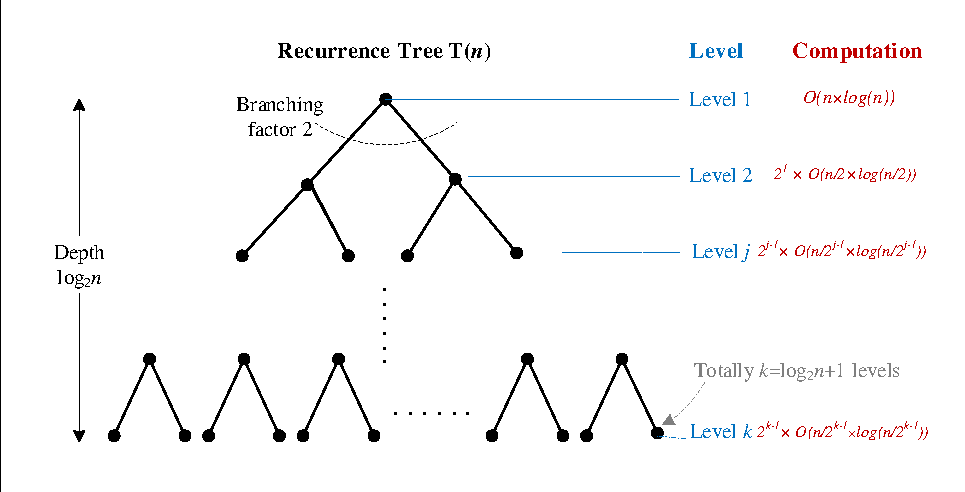
\includegraphics[width=0.8\textwidth]{Fig-RecurrenceTree.pdf}
    \caption{Recurrence Tree}\label{Fig-RecurrenceTree}
\end{figure}

The time complexity of the algorithm is the summation of each level's time complexity, which is 
\begin{equation}
\begin{split}
T(n)&=cn\log n+ 2\times c\frac{n}{2} \log \frac{n}{2}+\cdots +2^{k-1}\times c\frac{n}{2^{k-1}}\log \frac{n}{2^{k-1}}\\
&=cn \log( n \times \frac{n}{2} \times \frac{n}{2^2} \times \cdots\times\frac{n}{2^{k-1}})\\
&=cn\log \frac{n^{\log_2 n+1}}{2^{\frac{(\log_2 n+1)(\log_2 n)}{2}}}\\
&=cn\log n^{\frac{\log_2 n+1}{2}}\\
&=cn\log n^{\frac{\log_2 n}{2}}+cn\log \sqrt{n}\\
&=\frac{c}{2\log 2}n \log^2 n+cn\log\sqrt{n}\\
&=O(n\log^2 n)
\end{split}
\end{equation}
Thus, the time complexity of the algorithm is $O(n\log^2 n)$.

\item We \emph{can not} use plain master theorem to solve this problem because the exact time complexity of the algorithm is not any format of the master theorem's possible results.

However, we could get the generalization of master theorem from the book \textit{Induction to Algorithms}:\\
In the equation $$T(n)=aT(n/b)+f(n)$$ satisfies 
$$f(n)=\Theta(n^{\log_b a}\log^k n)\quad and\quad k\geq 0$$
the solution of the equation is $$T(n)=\Theta(n^{\log_b a}\log^{k+1} n)$$, which could be applied to the problem.

\end{enumerate}
\end{solution}
\item
\textit{Transposition Sorting Network.} A comparison network is a \textbf{transposition network}  if each comparator connects adjacent lines, as in the network in Fig.~\ref{Fig-Transposition}.

\begin{figure}[htbp]
    \centering
    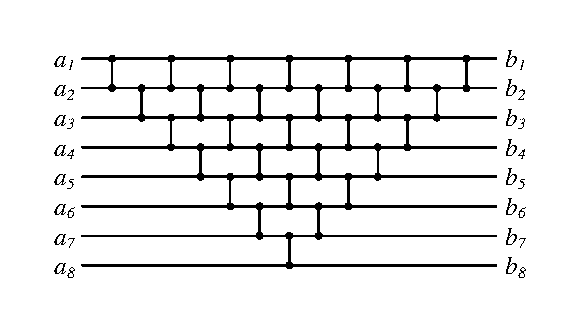
\includegraphics[width=0.4\textwidth]{Fig-Transposition.pdf}
    \caption{A Transposition Network Example}\label{Fig-Transposition}
\end{figure}


\begin{enumerate}
\item Prove that a transposition network with $n$ inputs is a sorting network if and only if it sorts the sequence $\langle n, n-1, \cdots, 1 \rangle$. {\color{blue}(Hint: Use an induction argument analogous to the \emph{Domain Conversion Lemma}.)}
\item {\color{red}{(Optional Sub-question with Bonus)}} Given any $n \in \mathbb{N}$, write a program using Tkinter in Python to draw a figure similar to Fig.~\ref{Fig-Transposition} with $n$ input wires.
\end{enumerate}
\end{enumerate}
\begin{enumerate}
\item
\begin{solution}
~\\
Before the beginning of our proof of the problem, let we prove a lemma. 
\begin{lemma}
There is a transposition network with any input sequence $<a_1,a_2,\cdots,a_n>$, of which the maximum is denoted as $max_a$. If the comparators that make the $max_a$ going down are all deleted, whichever wire the $max_a$ is on initially, the rest of the network will remain the same.\\ (\textbf{Definition of the delete operation:}) As is shown in ~\ref{Fig-DeleteExample}, if the input is $<x,y>$ where $x\leq y$, the comparator is deleted and the down-left node and the upper-right node is connected. At the same time, $x$ is dropped and the output size is smaller than the input size by $1$.)
\begin{figure}[htbp]
    \centering
    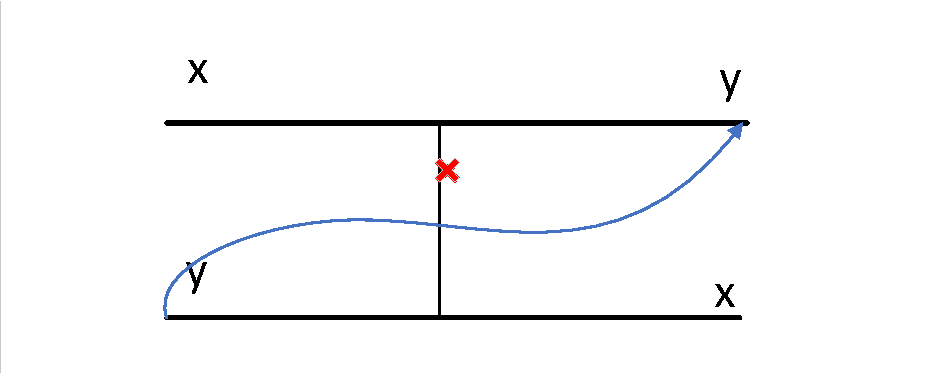
\includegraphics[width=0.8\textwidth]{Fig-DeleteExample.pdf}
    \caption{Delete Operation Example}\label{Fig-DeleteExample}
\end{figure}
\begin{proof}[Proof of the lemma 1]
~\\
\textbf{Basis step:} The $n=2$ case is proved by the definition of the delete operation. \\
\textbf{Induction hypothesis:} Assume that for the input size of $n$, if the comparators that make the $max_a$ going down are all deleted, whichever wire the $max_a$ is on initially, the rest of the network will remain the same.\\
\textbf{Proof of induction step:} For the input size of $n+1$, the rest of $n$ wires above remains the same. The comparator between the $n$ and $n+1$ wires is the basis situation, so the lemma is proved yet.

\end{proof}
\end{lemma}
.\\
{\Large \textbf{Proof of the original problem:}}\\
\textbf{Basis step:} For $n=2$, the transposition network composes only one comparator and it is obviously true.
\\
\textbf{Induction hypothesis:} Assume that the transposition network which could sort the input sequence of $<n,n-1,\cdots,1>$ could sort any sequence. 
\\
\textbf{Proof of the induction step:} For the transposition network which could sort the input sequence of $<n+1,n,\cdots,1>$, if the wire the maximum of the input sequence $n+1$ going down is deleted, the rest of the network could sort the input sequence of $<n,n-1,\cdots,1>$, which could sort any sequence according to the induction hypothesis, as is shown in the Fig.~\ref{Fig-BigDeleteExample}.

\begin{figure}[htbp]
    \centering
    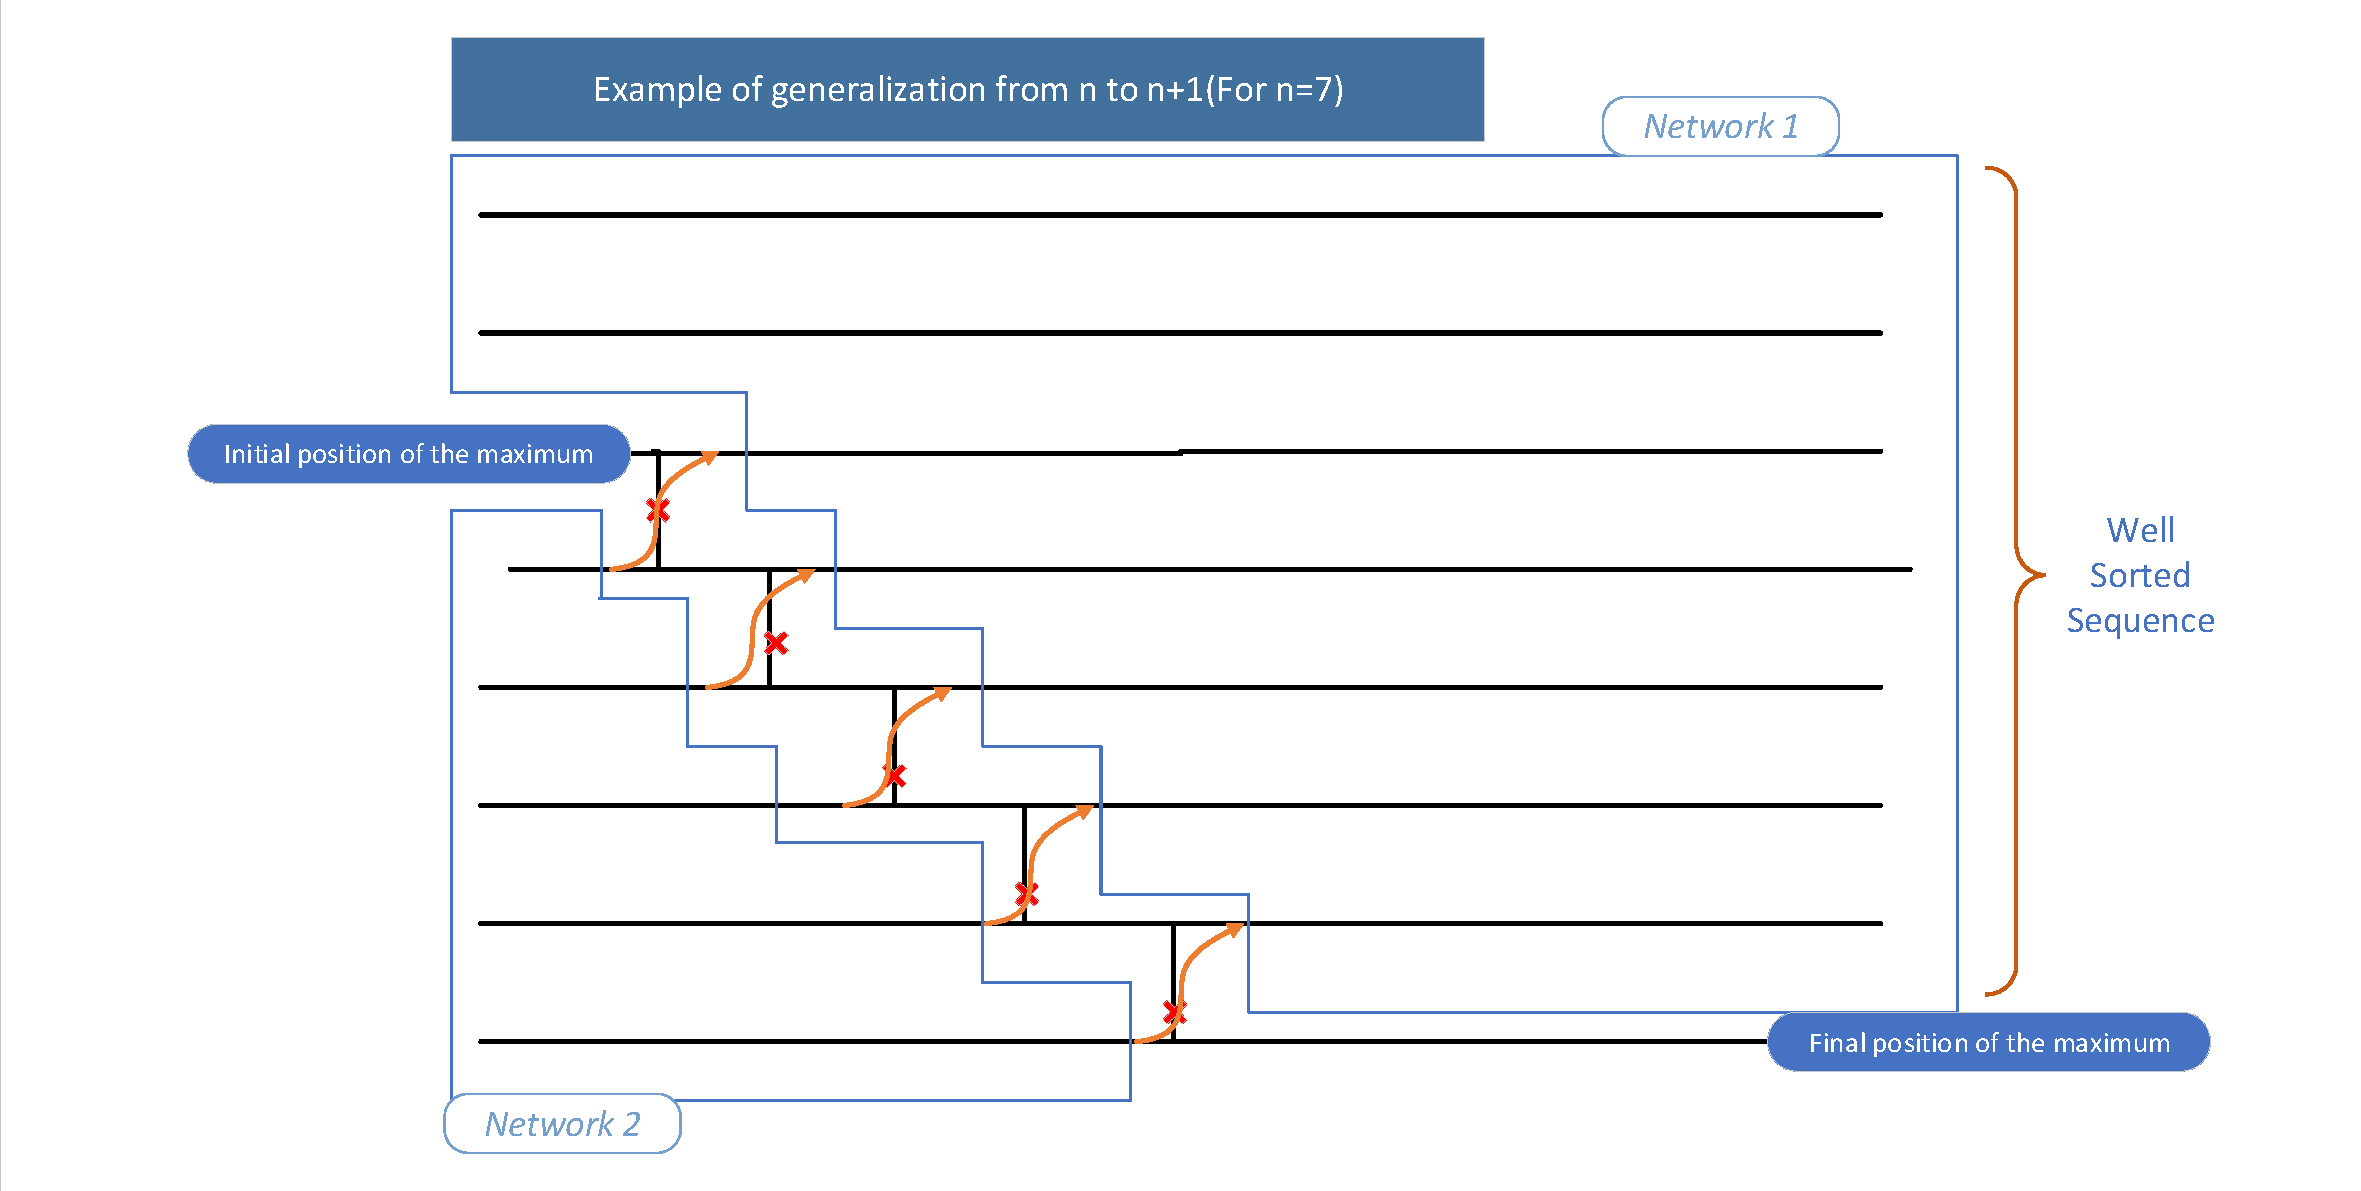
\includegraphics[width=0.8\textwidth]{Fig-BigDeleteExample.pdf}
    \caption{Example of generalization from n to n+1(For n=7)}\label{Fig-BigDeleteExample}
\end{figure}

Because the network could sort the sequence $<n+1,n,\cdots,1>$, there must be a comparator between every adjacent lines and the maximum of the input sequence will go down to the bottom line along these comparators. 

According to the \textit{Lemma 1}, if we delete the path the maximum of the input sequence going down, the rest of the network will remain the same, which is $n$ case in the induction hypothesis and can sort the other numbers of the input except for the maximum. At the same time, the maximum is on the bottom line eventually, so the network could sort any input sequence with the size of $n+1$. 
\end{solution}
\item
The source code is in file \textit{Code.py} and you must execute it with \textbf{python3}. The content of the code is shown in Fig.
Fig.~\ref{fig:res} shows the output of the program when $n=8$ and $n=9$. However, you could input any integer as you like.

\begin{figure}
%\begin{tabular}{cc}   
\begin{minipage}{0.5\linewidth}
  \centerline{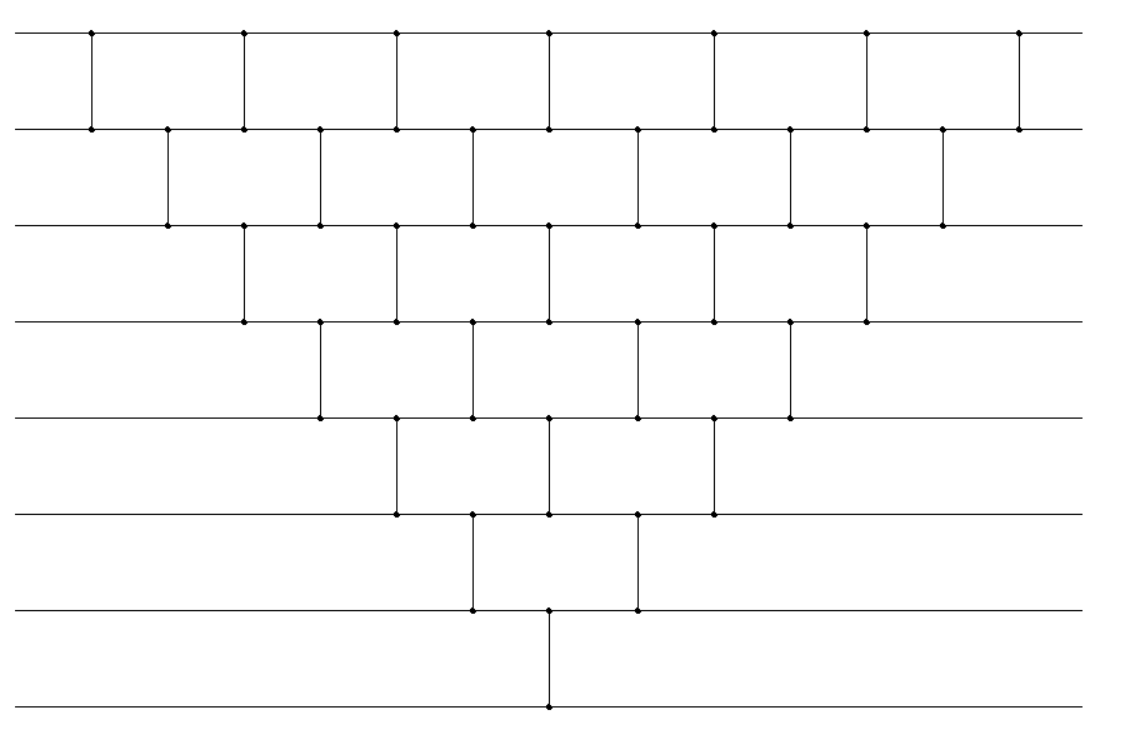
\includegraphics[width=6.0cm]{Fig-EXAMPLE8.png}}
  \centerline{(a) $n=8$ }
\end{minipage}
\hfill
\begin{minipage}{0.5\linewidth}
  \centerline{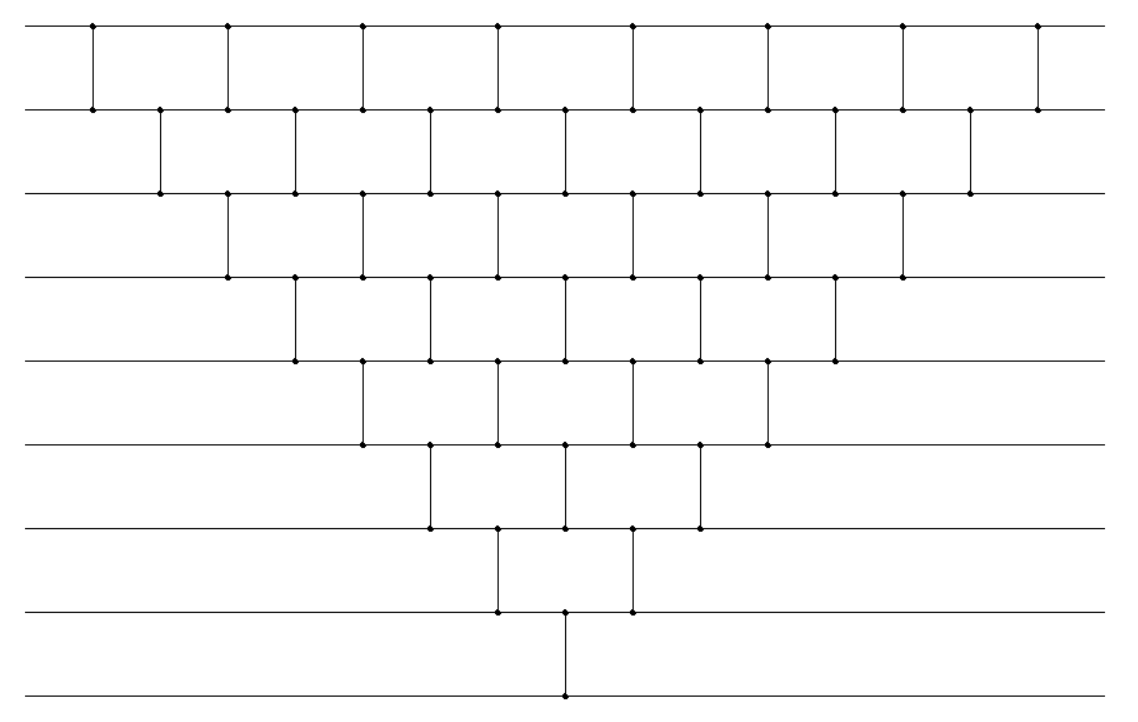
\includegraphics[width=6.0cm]{Fig-EXAMPLE9.png}}
  \centerline{(b) $n=9$}
\end{minipage}
\hfill
%\end{tabular}
\caption{Example of the transposition network.}
\label{fig:res}
\end{figure}
\begin{figure}[htbp]
    \centering
    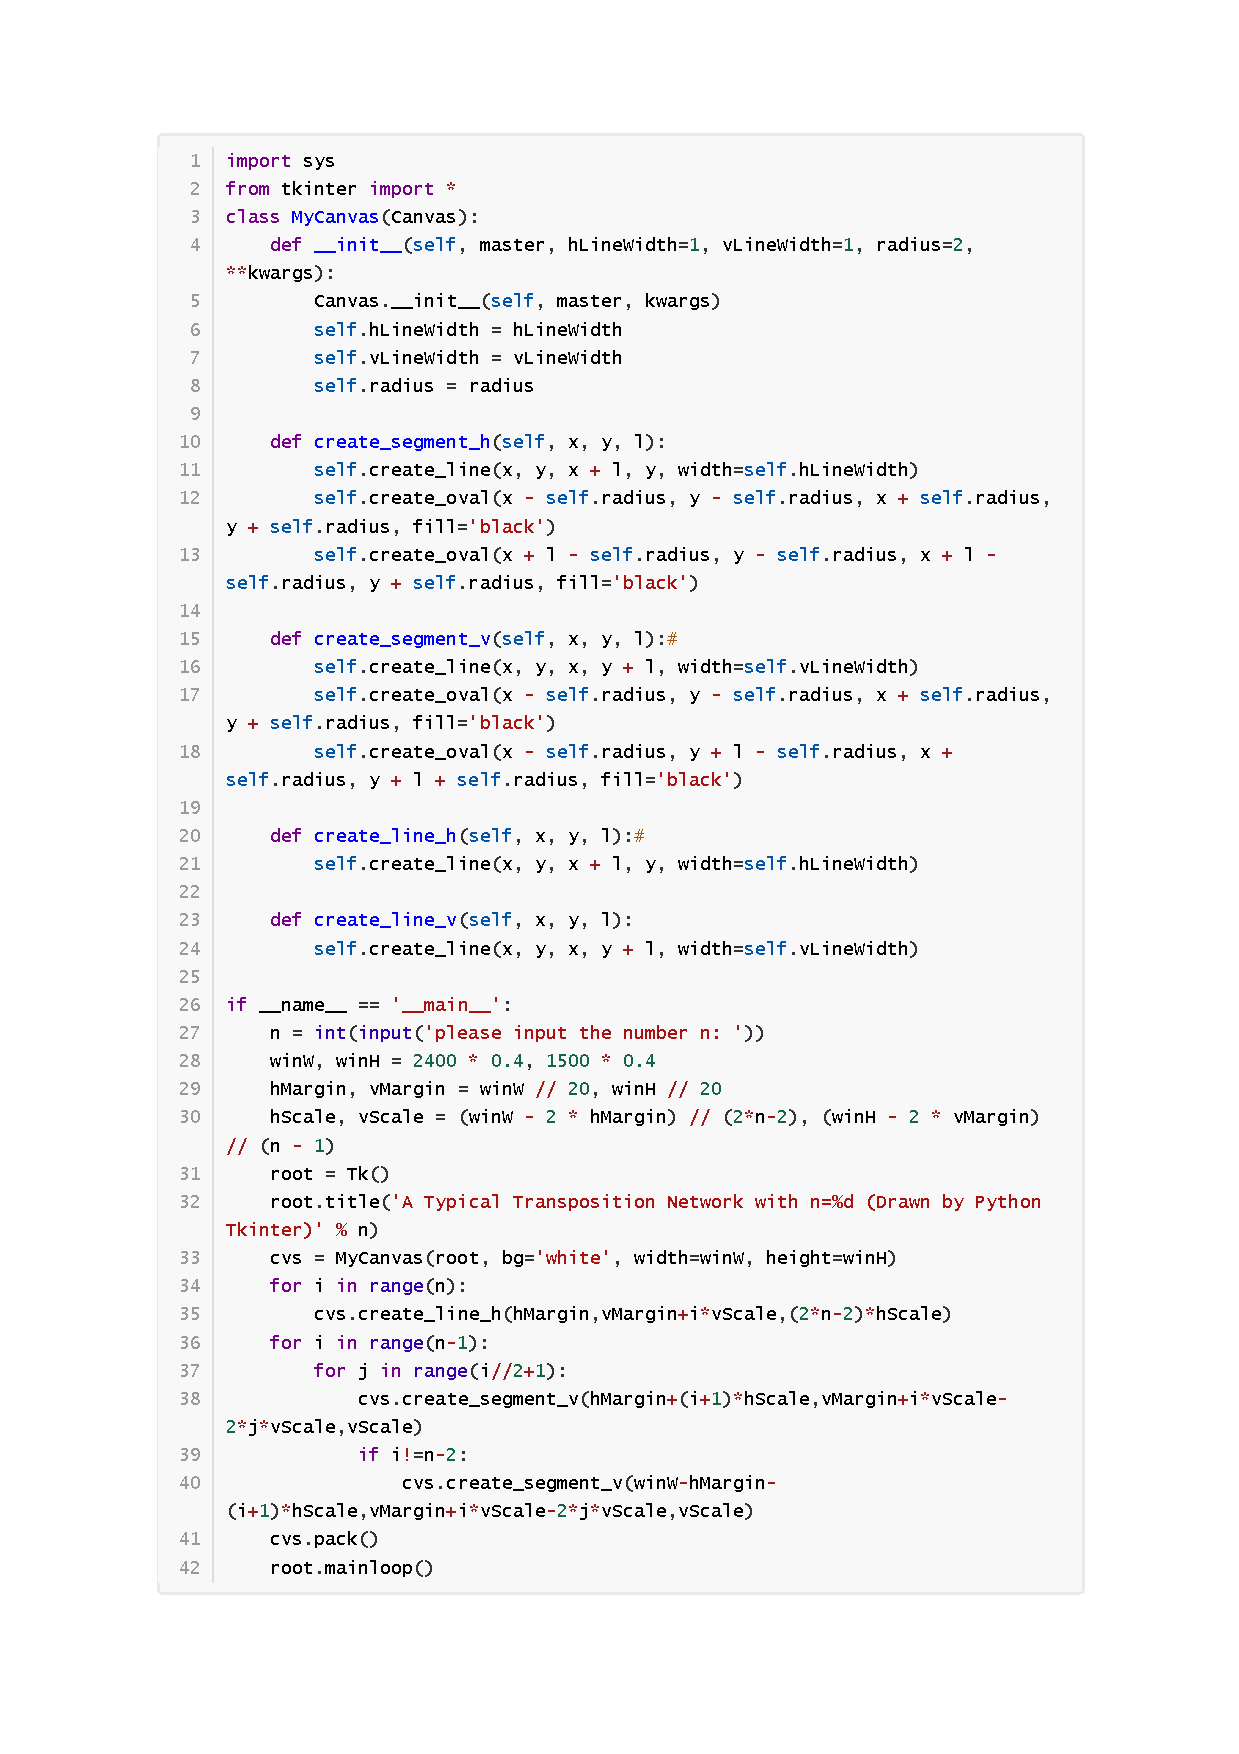
\includegraphics[width=1\textwidth]{Fig-Code.pdf}
    \caption{Source code}\label{Fig-Code}
\end{figure}
\end{enumerate}

%========================================================================
\end{document}
